\documentclass[a4,12pt]{horizon-theme}
\usepackage{enumitem}
\usepackage{cleveref}

\setTitle{Segmentação de Imagens de Raio-X do Pulmão usando Redes Neurais Convolucionais}
\setUniversity{Universidade de São Paulo}
\setFaculty{Escola Politécnica}
\setDepartment{Departamento de Eng. da Computação e Sist. Digitais}
\setCoverMainLogo{figures/minerva.pdf}

\setCoverLeftBox{%
  {\Large Projeto Final}\\[2pt]
  {PTC5892 -- Processamento de Imagens Médicas}\\[75pt]
  {\Large Natanael Magalhães Cardoso}\\[10pt]
  {\large \textsc{Professor:} Prof. Dr. Sergio S. Furuie}
}

\setCompactAuthors{Natanael Magalhães Cardoso\textsuperscript{{\large $\star$}, \faEnvelope[regular]}%,%
%, Prof. Cláudia Mendes de Oliveira\textsuperscript{$\dagger$}}
% { } Prof. Dr. Antonio Mauro Saraiva\textsuperscript{{\large $\star$}, $\dagger$}}
}

\setHeaderRight{N. M. Cardoso}
\setHeaderLeft{Escola Politécnica}

\setCompactInfo{\textsuperscript{\large $\star$} {\small Departamento de Engenharia de Computação e Sistemas Digitais, Escola Politécnica, Universidade de São Paulo.}\\[10pt]
% \textsuperscript{$\dagger$} {\small Orientador}\\[10pt]
% \textsuperscript{$\dagger$} {\small Departamento de Astronomia, Instituto de Astronimia, Geofísica e Ciências Atmosféricas, Universidade de São Paulo.}\\[10pt]
\textsuperscript{\faEnvelope[regular]} {\small contato@natanael.net}\\[10pt]
{\color{gray}\rule{\linewidth}{0.4pt}}\\[10pt]
{\bf Palavras-chave:} base de conhecimento, visão computacional, vision transformers, aprendizagem profunda, processamento de imagens médicas, raio-X, segmentação.}

\setAbstract{Este trabalho aborda o desenvolvimento e avaliação de um modelo baseado em Redes Neurais Convolucionais (CNNs) para a segmentação de imagens de raio-X do pulmão. O estudo avalia a aplicação de técnicas de Aprendizado Profundo (DL), como a Transferência de Aprendizagem e o Aumento Artificial de Dados, explorando a arquitetura EfficientUNet. O objetivo é desenvolver um modelo que, a partir das imagens de raio-X, faça a predição da segmentação tando do pulmão quanto da infecção de Covid-19, em duas imagens distintas. Na avaliação do modelo no conjunto de teste, foi obtido 91,35\% e 88,46\% na métrica de similaridade estrutural (SSIM) para imagens de segmentação do pulmão e da infecção, respectivamente.}

% \setAbstract{Este trabalho apresenta uma abordagem inovadora para criar uma base de conhecimento para busca por similaridade visual, utilizando embeddings gerados pelo modelo MaxViT, um transformer de visão, em conjunto com o algoritmo HNSW para fornecer uma interface web eficaz e acessível. O MaxViT, uma variação do Transformer, demonstrou excelentes resultados na extração de representações visuais de alta qualidade, enquanto o HNSW possibilita uma busca rápida e escalável dentro do espaço de embeddings. Essa combinação oferece uma base de conhecimento robusta e eficiente, capacitando os usuários a explorarem vastos conjuntos de dados visuais de maneira intuitiva e precisa. A interface web desenvolvida oferece uma experiência de busca visualmente rica, permitindo aos usuários carregar uma imagem de consulta ou fornecer uma descrição textual para recuperar imagens semelhantes a partir do banco de dados.} %Com recursos como visualização de resultados, filtragem por categoria e personalização de preferências de busca, a interface torna a busca por imagens uma experiência altamente interativa e envolvente %Além disso, a acessibilidade universal da plataforma, que pode ser acessada de qualquer dispositivo conectado à Internet, amplia seu alcance e utilidade, proporcionando uma solução flexível e conveniente para a exploração de conteúdo visual.}

% Contudo, uma classificação morfológica feita através de inspeção visual está sujeita a um viés causado pela subjetividade da observação humana. Neste trabalho,  propomos um modelo de \emph{Deep Learning} treinado a partir de classificações visuais do GalaxyZoo e imagens do Legacy Survey. O objetivo é obter um modelo de \emph{Deep Learning} que seja capaz de classificar galáxias mergers com magnitude $r < 17.5$}



\definecolor{myred}{rgb}{0.99, 0.14, 0.12}
\newcommand{\natanael}[3]{{\fcolorbox{myred}{myred}{\color{white}Item #1:}} {\color{myred}\sout{#2}} {\color{myred} #3}}


\newcolumntype{Y}{>{\raggedleft\arraybackslash}X}
% \rowcolors{2}{blue!5!white}{blue!15!white}
\newtcolorbox[blend into=tables]{htable}[4]{%
    enhanced,
    fonttitle=\bfseries,
    colback=white,
    colframe=secondaryColor!90!white,
    colbacktitle=secondaryColor!90!white,
    coltitle=white,
    center title,
    halign title=center,
    toptitle=40pt,
    bottomtitle=40pt,
    boxrule=.8pt,
    float=!htb,
    title=\strut {#2},
    tabularx*={\arrayrulewidth0.4mm\renewcommand{\arraystretch}{1.5}}{#1},
    before upper app={#3\\\hline\hline},
    label={#4},
}


\usepackage{translator}
\usepackage{pgfgantt}
\AtBeginEnvironment{ganttchart}{\deftranslation[to=Brazilian]{May}{Mai}}
\definecolor{barblue}{RGB}{153,204,254}
\definecolor{groupblue}{RGB}{51,102,254}


\addbibresource{refs.bib}
\begin{document}
\horizonCover

\horizonTitle

\horizonAbstract

\newpage

% \tableofcontents

% \newpage

\onehalfspacing
\section{Introdução}
A Apredizagem Profunda (DL, \cite{Goodfellow2016}) é uma segmento específico dentro da área de Aprendizado de Máquina (ML) e, por conseguinte, da área de Inteligência Artificial. Consiste no desenvolvimento de redes neurais artificiais que são combinadas em um número significativamente maior do que as redes neurais tradicionais. Este tipo de técnica se transformou no estado-da-arte do reconhecimento de padrões em imagens devido a um tipo específico de rede neural conhecida como convolucional.
As redes neurais convolucionais (CNNs, \cite{lecun2015deep}), são inspiradas e propostas com certa analogia ao processamento das imagens realizadas no córtex visual de mamíferos.

O processo começa quando um estímulo visual alcança a retina e equivale a um sinal que atravessa regiões específicas do cérebro. Essas regiões são responsáveis pelo reconhecimento de cada uma dessas características correspondentes \citep{karpathy2016convolutional}.
Os neurônios biológicos das primeiras regiões respondem pela identificação de formatos geométricos primários, enquanto neurônios das camadas finais têm a função de detectar características mais complexas, formadas pelas formas simples anteriormente reconhecidas \citep{vedaldi2015matconvnet}. Características com padrões muito específicos do objeto são estabelecidas depois que o procedimento se repete. De forma análoga, a CNN decompõe a tarefa de reconhecimento de um objeto em subtarefas. Para isso, durante a aprendizagem, a CNN divide a tarefa em subníveis de representação das características, posteriormente aprendendo a reconhecer novas amostras da mesma classe  \citep{lecun2015deep,vedaldi2015matconvnet}.
Desta forma, as CNNs são capazes de predizer características complexas sem a necessidade de um pré processamento e são invariantes â escala e à rotação dos dados, o que torna essencial a classificação em imagens.

As CNNs já são amplamente utilizadas em diversas áreas do conhecimento para resolver problemas relacionados a visão computacional, como classificação de software malicioso \citep{VGG16Ex01}, de plantas \citep{VGG16Ex02}, de imagens de satélite \citep{InceptionResNetV2Ex01} e até de músicas \citep{DenseNetEx05}. Na área médica, há uma vasta gama de utilização das CNNs, como a classificação de células cancerígenas \citep{InceptionResNetV2Ex03}, de tumores cerebrais \citep{VGG16Ex03}, de câncer de mama \citep{DenseNetEx01}, de esclerose múltipla \citep{DenseNetEx03} e de eletrocardiogramas \citep{EfficientNetEx01}.

Neste trabalho, será usada uma a arquitetura EfficientUnet para desenvolver um modelo que, a partir das imagens de raio-X, faça a predição da segmentação tando do pulmão quanto da infecção de Covid-19, em duas imagens distintas.


\section{Conjunto de Dados}
\label{sec:dados}
Para treinar o modelo, é usado um conjunto de dados de imagens de raio-X do pulmão compilado por pesquisadores de Qatar University \citep{CovidDataset1, CovidDataset2}. Este conjunto de dados contém 11.956 imagens de Covid-19, 11.263 imagens de outras infecções e 10.701 imagens de pacientes saudáveis. Cada elemento do conjunto é composto por três imagens: raio-X do paciente, segmentação do pulmão e segmentação da infecção.

Assim, dois grupos de imagens foram criados: covid e não-covid. O primeiro com as 11.956 imagens de Covid-19 e o segundo com as demais imagens. Subsequentemente, o conjunto de dados foi dividido em três subconjutos: treino (70\%), validação (15\%) e teste (15\%).







\section{Método}
\subsection{Arquiteturas de Redes Neurais}

\subsubsection{UNet}
\label{sec:unet}
\begin{figure}[!ht]
  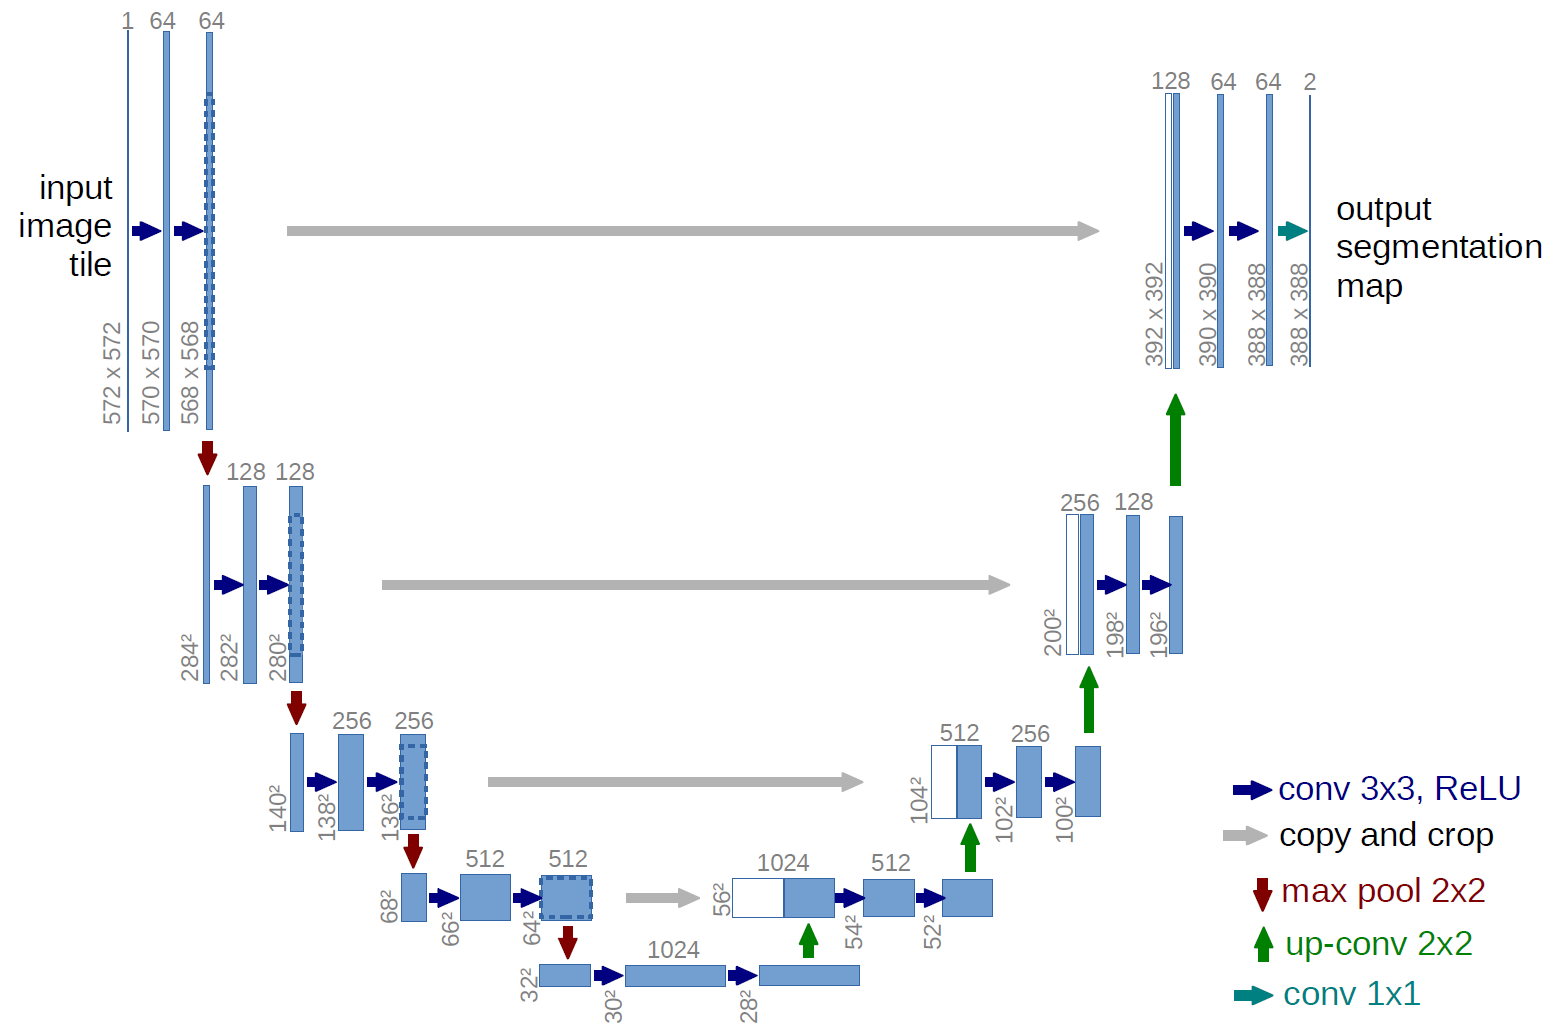
\includegraphics[width=\textwidth]{figures/unet.png}
  \caption{Arquitetura da Rede Neural Convolucional U-Net, criada para segmentação de imagens médicas. Fonte: \textsc{Ronneberger et al., 2015}.}
  \label{fig:unet}
\end{figure}

A arquitetura de rede neural UNet, mostrada na Fig. \ref{fig:unet}, foi projetada para tarefas de segmentação semântica em imagens biomédicas, como a segmentação de células ou órgãos em imagens de microscopia \citep{unet}. Ela foi criada para resolver um dos principais desafios da segmentação de imagens: a necessidade de captar detalhes finos enquanto preserva a estrutura global da imagem.

A UNet é composta por duas partes principais: o caminho de contração (encoder) e o caminho de expansão (decoder). O primeiro é responsável por extrair características da imagem, utilizando uma sequência de camadas de convolução seguidas de funções de ativação (geralmente ReLU) e operações de pooling para reduzir gradualmente a resolução espacial da imagem, mas aumentar a profundidade da informação extraída. Essa seção é similar a outras arquiteturas de redes neurais convolucionais, como a VGG.

Após a extração das características, a UNet começa a expandir a imagem de volta à sua resolução original (decoder), utilizando operações de upsampling e convoluções. O diferencial é que, a cada etapa de upsampling, as informações extraídas em estágios equivalentes do encoder são concatenadas (skip connections) para ajudar na reconstrução detalhada da imagem segmentada.

A utilização de skip connections permite que a UNet combine a localização precisa de características espaciais da camada correspondente do encoder com as informações mais contextuais da camada do decoder, resultando em segmentações precisas mesmo em bordas finas ou estruturas complexas.

Comparada a arquiteturas de segmentação anteriores, a UNet é relativamente eficiente, requerendo menos dados anotados para alcançar bons resultados. Isso é crucial em contextos biomédicos onde anotar grandes quantidades de dados pode ser difícil e caro.

% Embora tenha sido criada para segmentação de imagens biomédicas, a UNet mostrou-se eficaz em várias outras tarefas de segmentação, como segmentação de imagens satelitais, processamento de imagens de ultrassom, e até mesmo em aplicações fora do domínio médico.


\subsubsection{EfficientNet}
\label{sec:effnet}
\begin{figure}[!ht]
  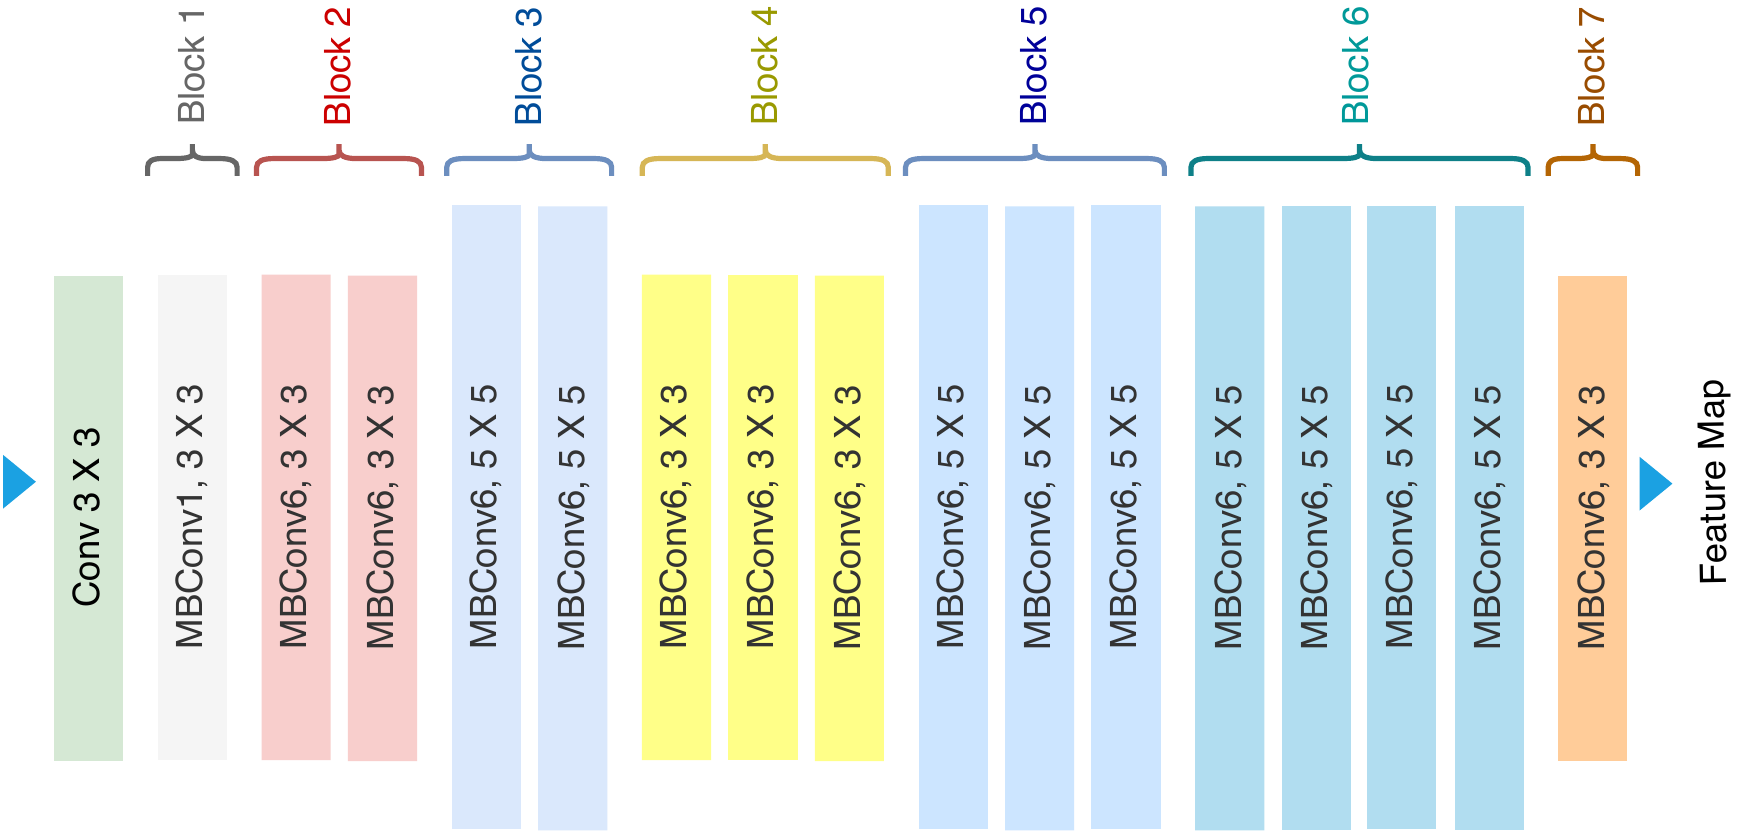
\includegraphics[width=\textwidth]{figures/EfficientNet.png}
  \caption{Arquitetura da Rede Neural Convolucional Efficient. Fonte: \textsc{Tan e Le, 2020}.}
  \label{fig:effnet}
\end{figure}
A arquitetura EfficientNet, proposta por \cite{EfficientNet} e mostrada na Fig. \ref{fig:effnet}, foi introduzida como uma abordagem para projetar CNNs mais eficientes em termos de desempenho e recursos computacionais. A principal inovação da EfficientNet é sua metodologia de escalonamento, que permite criar redes de diferentes tamanhos que mantêm um equilíbrio ótimo entre precisão e eficiência. O resultado é uma família de modelos (EfficientNet-B0 a EfficientNet-B7) que variam em tamanho e capacidade, mas mantêm uma eficiência notável em termos de precisão por FLOP (Floating Point Operation).

A EfficientNet baseia-se em um conceito chamado compound scaling, que propõe o escalonamento conjunto das três principais dimensões de uma rede neural: profundidade, largura e resolução da imagem de entrada. Em arquiteturas anteriores, o aumento do desempenho geralmente envolvia apenas uma dessas dimensões, o que poderia levar a um uso ineficiente dos recursos computacionais.

A profundidade refere-se ao número de camadas na rede. Aumentar a profundidade geralmente melhora a capacidade da rede de capturar características complexas, mas também aumenta o custo computacional e o risco de overfitting.

A largura refere-se ao número de filtros em cada camada. Aumentar a largura permite capturar mais informações em cada camada, mas também aumenta a quantidade de parâmetros e o custo computacional.

A resolução da imagem de entrada pode ser aumentada para capturar mais detalhes, mas isso também aumenta o custo computacional e o tempo de treinamento.

Ao equilibrar cuidadosamente a profundidade, a largura e a resolução, a EfficientNet oferece um desempenho superior com menos recursos computacionais em comparação com outras arquiteturas, como ResNet ou Inception. Desta forma, a EfficientNet pode ser ajustada para diferentes aplicações e limites de recursos, desde dispositivos móveis com capacidades limitadas até sistemas de ponta com recursos abundantes.


\subsubsection{EfficientUNet}
\label{sec:effunet}
\begin{figure}[!ht]
  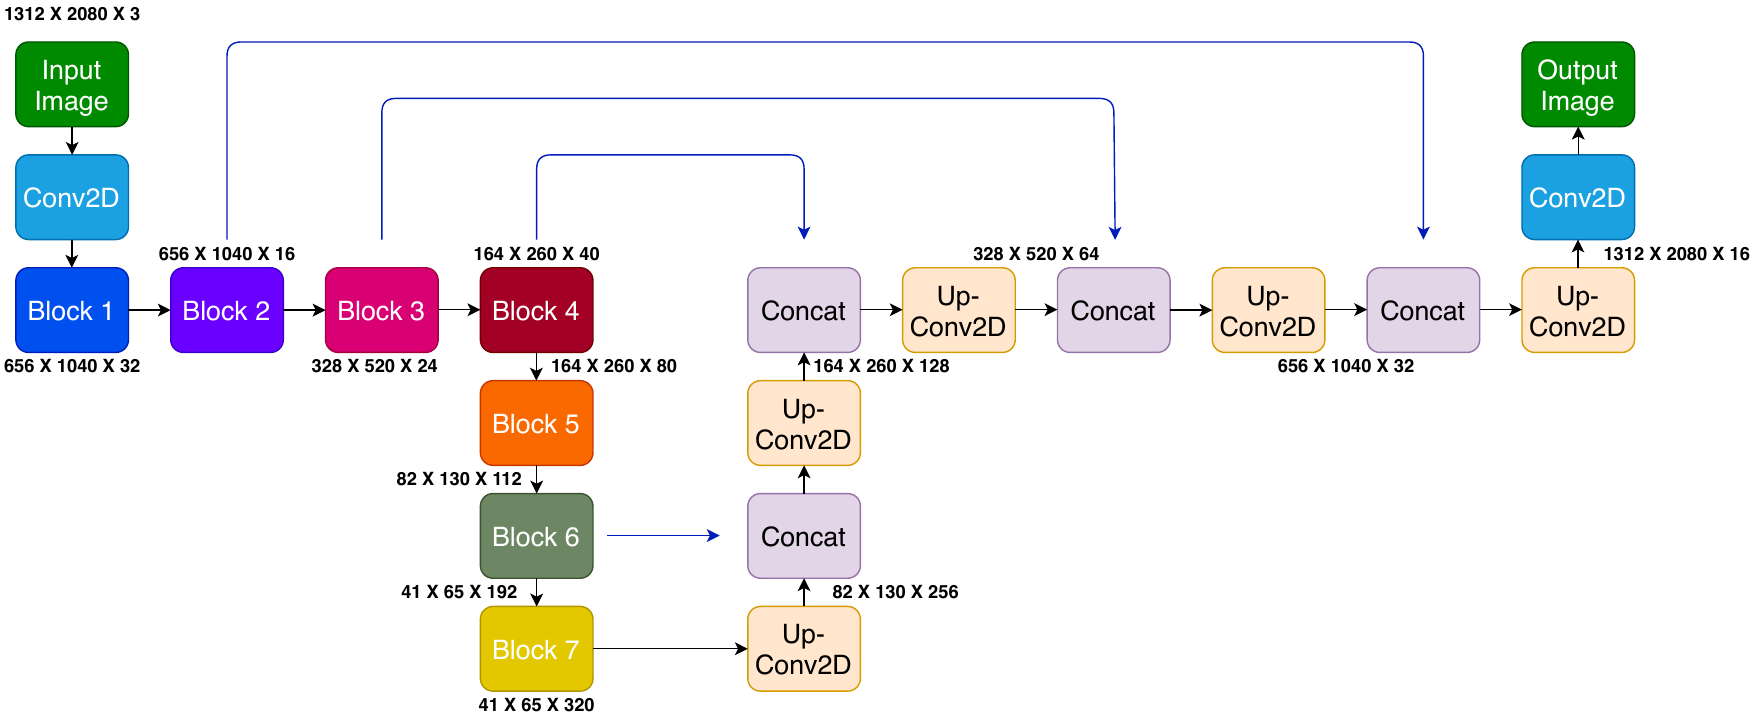
\includegraphics[width=\textwidth]{figures/EfficientUnet.png}
  \caption{Arquitetura da Rede Neural Convolucional EfficientUnet, criada para segmentação de imagens de satélite. Fonte: \textsc{Ahmed e Sabab, 2022}.}
  \label{fig:effunet}
\end{figure}

A arquitetura EfficientUNet, mostrada na Fig. \ref{fig:effunet}, é uma combinação das arquiteturas EfficientNet e UNet, projetada para melhorar a eficiência e a precisão em tarefas de segmentação de imagens, especialmente em contextos onde os recursos computacionais são limitados, mas a precisão é crucial \citep{effunet}. Essa arquitetura é projetada para cenários onde é necessário manter um bom desempenho com uso otimizado de recursos, como em dispositivos móveis ou em aplicações em tempo real.

A EfficientUNet utiliza a EfficientNet (Seção \ref{sec:effnet}) como a parte do encoder para extrair características da imagem de entrada. A EfficientNet é escolhida por sua eficiência computacional e capacidade de capturar representações ricas da imagem com menos parâmetros em comparação com outras arquiteturas tradicionais.

A parte do decoder segue a estrutura típica da UNet (Seção \ref{sec:unet}), onde as características extraídas são progressivamente aumentadas em resolução para reconstruir uma imagem segmentada. Como na UNet original, o decoder da EfficientUNet também incorpora skip connections entre as camadas correspondentes do encoder e do decoder, ajudando a preservar detalhes importantes da imagem.

Aproveitando a eficiência da EfficientNet, a EfficientUNet oferece um modelo leve e rápido, que é particularmente útil para implementações em dispositivos com recursos limitados, como dispositivos móveis ou sistemas embarcados.

A combinação da capacidade de extração de características da EfficientNet com o mecanismo de segmentação da UNet resulta em segmentações precisas, o que é crucial em tarefas que exigem alta exatidão, como na área médica. Este trabalho usa esta arquitetura para segmentar as imagens de raio-X do pulmão.



\subsection{Transferência de Aprendizagem}
\label{sec:tl}
A transferência de aprendizagem \citep{transfer} é uma técnica onde um modelo treinado em uma tarefa é reutilizado ou ajustado para uma nova tarefa. Ao invés de treinar um modelo do zero com um grande volume de dados, a transferência de aprendizagem permite aproveitar o conhecimento previamente adquirido em outra tarefa relacionada, o que pode acelerar o processo de treinamento e melhorar a performance do modelo, especialmente quando há limitação de dados.

A transferência de aprendizagem tem se tornado uma prática fundamental no treinamento de redes neurais convolucionais (CNNs), especialmente para tarefas de visão computacional como classificação, detecção de objetos e segmentação de imagens. Um dos principais motivos é que treinar uma CNN do zero requer grandes quantidades de dados rotulados e recursos computacionais consideráveis, o que nem sempre é viável.

Neste trabalho, será testada a inicialização dos pesos provenientes de uma rede pré-treinada usando a base de dados \emph{ImageNet}\footnote{\url{http://www.image-net.org/}} traz uma grande melhoria na precisão dos resultados da classificação. Essa base de dados possui milhões de imagens de objetos do cotidiano.


\subsection{Aumento Artificial de Dados}
\label{sec:dataaug}
Aumento artificial de dados \citep{Larry1996} é a aplicação de transformações afins nas imagens a cada época no conjunto de treinamento, por exemplo rotação, reflexão, translação e mudança de escala. As matrizes das equações (\ref{eq:rotation}, \ref{eq:reflection}, \ref{eq:translation} e \ref{eq:shear}) definem as transformações usadas.

A transformação $R(\theta)$ rotaciona a imagem por um ângulo $\theta$.

\begin{equation}\label{eq:rotation}
  \begin{gathered}
    R(\theta) =
    \begin{bmatrix}
      \cos(\theta) & -\sin(\theta) & 0 \\
      \sin(\theta) & \cos(\theta)  & 0 \\
      0            & 0             & 1
    \end{bmatrix}
  \end{gathered}
\end{equation}

A Transformação $H$ faz a reflexão horizontal da imagem.

\begin{equation}\label{eq:reflection}
  H =
  \begin{bmatrix}
    1 & 0  & 0 \\
    0 & -1 & 0 \\
    0 & 0  & 1
  \end{bmatrix}
\end{equation}

A transformação $T(x, y)$ aplica translação por $x$ pixel na direção horizontal e $y$ pixels na direção vertical.

\begin{equation}\label{eq:translation}
  T(x, y) =
  \begin{bmatrix}
    1 & 0 & -x \\
    0 & 1 & -y \\
    0 & 0 & 1
  \end{bmatrix}
\end{equation}

A transformação $S(x, y)$ aplica cisalhamento na imagem.

\begin{equation}\label{eq:shear}
  S(x, y) =
  \begin{bmatrix}
    1 & x & 0 \\
    y & 1 & 0 \\
    0 & 0 & 1
  \end{bmatrix}
\end{equation}

As transformações nas imagens são feitas remapeando as coordenadas dos píxeis originais aplicando uma combinação das matrizes das equações (\ref{eq:rotation}, \ref{eq:reflection}, \ref{eq:translation} e \ref{eq:shear}) em cada píxel da imagem original usando a equação \eqref{eq:final-transformation}, onde $M$ é a matriz das transformações combinadas, calculada a partir da multiplicação das matrizes de transformação anteriores, $(x, y)$ a coordenada do píxel da imagem original e $(x^*, y^*)$ a coordenada transformada do píxel.

\begin{align} \label{eq:final-transformation}
  \begin{bmatrix}
    x^* \\
    y^* \\
    1
  \end{bmatrix}
  =
  \ M\
  \begin{bmatrix}
    x \\
    y \\
    1
  \end{bmatrix}
\end{align}

Além disso, ainda é aplicada uma interpolação bilinear como \emph{anti-aliasing} \citep{aliasing, bilinear}. Durante o treinamento da rede, novas imagens de entrada são geradas a cada época a partir da transformação das imagens originais. Diversas transformações podem ser geradas substituindo $M$ da equação por combinações (multiplicação matricial) das transformações das equações (\ref{eq:rotation}, \ref{eq:reflection}, \ref{eq:translation} e \ref{eq:shear}). Tais transformações não mudam a interpretação da classe da imagem original, pois o espaço visual é invariante a elas. Logo, o objetivo de aplicar estas transformações nas imagens de entrada da rede é deixar que o algorítmo infira tal invariância, criando, assim, uma ``noção'' do espaço visual, o que resulta no aumento do potencial de generalização da rede \citep{Simard2003, CholletBook}. Frequentemente são relatados bons resultados com o uso desta técnica \citep{EfficientNetEx01, EfficientNetEx02, CNNEx04}, principalmente quando existe grande similaridade entre as classes.





\subsection{Hiperparâmetros}
\label{section:hyperparam}

Nesta seção descrevemos as definições dos principais conceitos, no contexto de aprendizagem profunda, que serão úteis para o entendimento dos métodos aqui utilizados. A função de ativação, função de custo, o otimizador, o learning rate, o número de épocas, além do número de camadas dos modelos, são importantes parâmetros responsáveis pela contrução do modelo definido a seguir.

\begin{description}
  \item[Função de ativação] \hfill \\
        A função de ativação é responsável por adicionar não-linearidade à rede. Sem ela, a saída de uma camada seria apenas uma transformação linear dos dados de entrada e a rede não seria beneficiada pelo empilhamento de diversas camadas lineares, pois isso não aumentaria o espaço de hipóteses. Logo, a função de ativação viabiliza representações mais complexas da rede, uma vez que define a complexidade de um modelo e, consequentemente, sua capacidade de generalização \citep{CholletBook}. Neste trabalho, a função $\rm{ReLU}(x) := \rm{max}(0, x)$ é usada nas camadas densas dos classificadores, a equação tangente hiperbólica é usada nas camadas densas do meta-modelo e a função Softmax \citep{Bridle1990} foi usada na última camada, tanto dos classificadores quanto do meta-modelo.

  \item[Função de Custo] \hfill \\
        A função de custo é utilizada com o objetivo de determinar o quão longe o modelo está do esperado, definindo a necessidade de atualização dos pesos da rede. Utilizamos a função Entropia Cruzada (\emph{Cross-Entropy})
        \begin{equation}
          \label{eq:custo}
          J({\bf w}) = -\frac{1}{N}\sum_{n=1}^N\left[ y_n\log \hat y_n + (1 - y_n)\log (1 - \hat y_n) \right]
        \end{equation}
        onde $y_n$ representa a probabilidade da classe dada pelo conjunto de treinamento do objeto $n$ e $\hat{y}_n$ representa a previsão da rede para este mesmo objeto.

  \item[Otimizador] \hfill \\
        O otimizador é um algorítmo iterativo com objetivo de minimizar a função de custo. Uma escolha típica é o método de gradiente descente e suas demais variações. Este tipo de algoritmo tem um parâmetro livre relacionado ao passo da iteração conhecido como taxa de aprendizado ou \textit{learning rate}. Neste trabalho foram testados diversos algoritmos considerados como estado-da-arte dos otimizadores como Adam \citep{Adam}, NAdam \citep{NAdam}, RAdam \citep{RAdam} e RMSprop \citep{RMSprop}.

  \item[Número de Épocas] \hfill \\
        O Número de épocas se referem a quantidade de vezes que o dataset de treino foi utilizado completamente no processo de otimização iterativa da função de custo. Um número de épocas adequado é necessário para que a função de custo seja minimizada.

  \item[Tamanho do Batch] \hfill \\
        O processo de otimização acontece em batches, cada iteração para minimizar a função custo é realizada com um número fixo de amostras, quando todas as amostras de treino são utilizadas se completa uma época.

  \item[Unidades de neurônios na última camada]
        \hfill \\
        A última camada da rede antes da camada de saída é responsável por condensar toda a informação extraída da rede para o processo de classificação final. Por esta razão, a quantidade de neurônios nessa camada pode ser particularmente sensível para a performance da rede. Neste trabalho utilizamos diferentes valores de neurônios para encontrar a quantidade que pode gerar a melhor performance.

  \item[Dropout]
        \hfill \\
        \emph{Dropout} \cite{dropout} é uma técnica de regularização muito utilizada em redes neurais por seu bom desempenho e baixo custo computacional. Aplicar esta regularização em uma camada consiste em eliminar aleatoriamente uma taxa dos neurônios de saída desta camada durante o treinamento, sendo geralmente escolhido um valor entre 0.2 e 0.5 para esta taxa \cite{CholletBook}.
\end{description}



\subsection{Treinamento}
\label{sec:treinamento}
Quatro diferentes modelos foram treinados usando diferentes técnicas de aprendizagem de máquina apresentadas nessa Seção. A Tabela \ref{tab:modelos} sumariza as técnicas empregadas  para o treinamento de cada modelo. Na próxima Seção, será discutida a melhora de desempenho com a aplicação de cada uma das técnicas.

\begin{table}[!ht]
  \centering
  \caption{Relação de modelos treinados}
  \label{tab:modelos}
  \begin{tabular}{lp{0.8\linewidth}}
    \toprule
    Modelo   & Método                                                                                                                             \\
    \hline
    Baseline & Modelo treinado com inicialização aleatória de pesos                                                                               \\
    Dataaug  & Modelo treinado com aumento artificial de dados (Seção \ref{sec:dataaug})                                                          \\
    ImageNet & Modelo treinado com transferência de aprendizagem (Seção \ref{sec:tl})                                                             \\
    Todos    & Modelo treinado com aumento artificial de dados (Seção \ref{sec:dataaug}) e com transferência de aprendizagem (Seção \ref{sec:tl}) \\
    \bottomrule
  \end{tabular}
\end{table}

\newpage
\subsection{Métricas de Avaliação}
\label{sec:metricas}

\subsubsection{Coeficiente de Dice}
Coeficiente de Dice é uma métrica utilizada para avaliar a similaridade entre duas amostras, sendo amplamente empregada em tarefas de segmentação de imagens. Sua definição é expressa na eq. \eqref{eq:dice}.

\begin{equation}\label{eq:dice}
  Dice(A, B) = \frac{2||A \cap B||}{||A|| + ||B||}
\end{equation}

onde $||A \cap B||$ é o número de elementos (ou pixels) que estão na interseção das duas amostras (conjunto de predições e conjunto de verdadeiros positivos), enquanto $||A||$  e $||B||$ são os tamanhos dos conjuntos predito e real, respectivamente.

O Coeficiente de Dice mede a sobreposição entre a segmentação prevista pelo modelo e a segmentação real (referência). Ele varia de 0 a 1, onde 0 indica nenhuma sobreposição e 1 indica sobreposição perfeita. Essa métrica é particularmente útil em segmentação de imagens porque leva em consideração tanto a precisão quanto a sensibilidade, oferecendo uma visão equilibrada de quão bem o modelo está performando.

Sendo assim, o Coeficiente de Dice mede a similaridade espacial entre a segmentação prevista e a segmentação real, ou seja, quão bem as regiões identificadas pelo modelo correspondem às regiões reais na imagem. Em outras palavras, é uma medida de acurácia espacial, que avalia a qualidade da segmentação realizada pelo modelo em termos de sobreposição entre as áreas previstas e as áreas verdadeiras.

\subsubsection{Índice de Jaccard}
O Índice de Jaccard, também conhecido como Coeficiente de Jaccard ou \emph{Intersection over Union} (IoU), é uma métrica utilizada para avaliar a similaridade entre dois conjuntos, sendo amplamente empregada na avaliação de modelos de segmentação de imagens. Essa métrica oferece uma medida clara e intuitiva da sobreposição entre a segmentação prevista pelo modelo e a segmentação real. Quanto maior a sobreposição entre as regiões previstas e as reais, maior o valor do IoU, que varia de 0 a 1, onde 0 indica nenhuma sobreposição e 1 indica sobreposição perfeita. Dessa forma, sua definição é a razão entre a interseção dos conjuntos A e B e a união dos mesmos, como mostra a eq. \eqref{eq:iou}.

\begin{equation}\label{eq:iou}
  Jaccard(A, B) = IoU(A, B) = \frac{||A \cap B||}{||A \cup B||}
\end{equation}

onde $||A \cap B||$ é o número de elementos (ou pixels) na interseção entre o conjunto de predições e o conjunto de verdadeiros positivos, e $||A \cup B||$ é o número total de elementos presentes na união dos conjuntos predito e real.

\subsubsection{Índice de Similaridade Estrutural}
O Índice de Similaridade Estrutural (ou \emph{Structural Similarity Index, SSIM}) é uma métrica utilizada para medir a similaridade perceptual entre duas imagens. Diferente de métricas tradicionais como MSE (\emph{Mean Squared Error}) ou PSNR (\emph{Peak Signal-to-Noise Ratio}), que avaliam a diferença ponto a ponto entre duas imagens, o SSIM é projetado para capturar as diferenças estruturais percebidas, considerando fatores como luminância, contraste e estrutura.

\begin{equation}\label{eq:ssim}
  SSIM(x, y) = \frac{(2\mu_x\mu_y + c_1)(2\sigma_{xy} + c_2)}{(\mu_x^2 + \mu_y^2 + c_1)(\sigma_x^2 + \sigma_y^2 + c_2)}
\end{equation}

onde $\mu_x$ e $\mu_y$ são as médias das intensidades das janelas $x$ e $y$; $\sigma_x^2$ e $\sigma_y^2$ são as variâncias das intensidades; $\sigma_{xy}$ é a covariância entre $x$ e $y$; $c_1$  e $c_2$ são constantes para estabilizar a divisão.



\section{Resultados}
O modelo EfficientUnet (Seção \ref{sec:effunet}) foi treinado no conjunto de treinamento e avaliado no conjunto de validação (informações sobre esses conjuntos estão na Seção \ref{sec:dados}). Durante o treinamento, foram monitoradas as métricas de avaliação definidas na Seção \ref{sec:metricas} e estão dispostas na Fig. \ref{fig:eval}, que mostra a evolução do treinamento para os modelos definidos na Seção \ref{sec:treinamento}: \emph{baseline}, \emph{dataaug}, \emph{imagenet} e \emph{todos}. É possível verificar que o modelo apresenta uma boa capacidade de generalização.

\begin{figure}[!ht]
  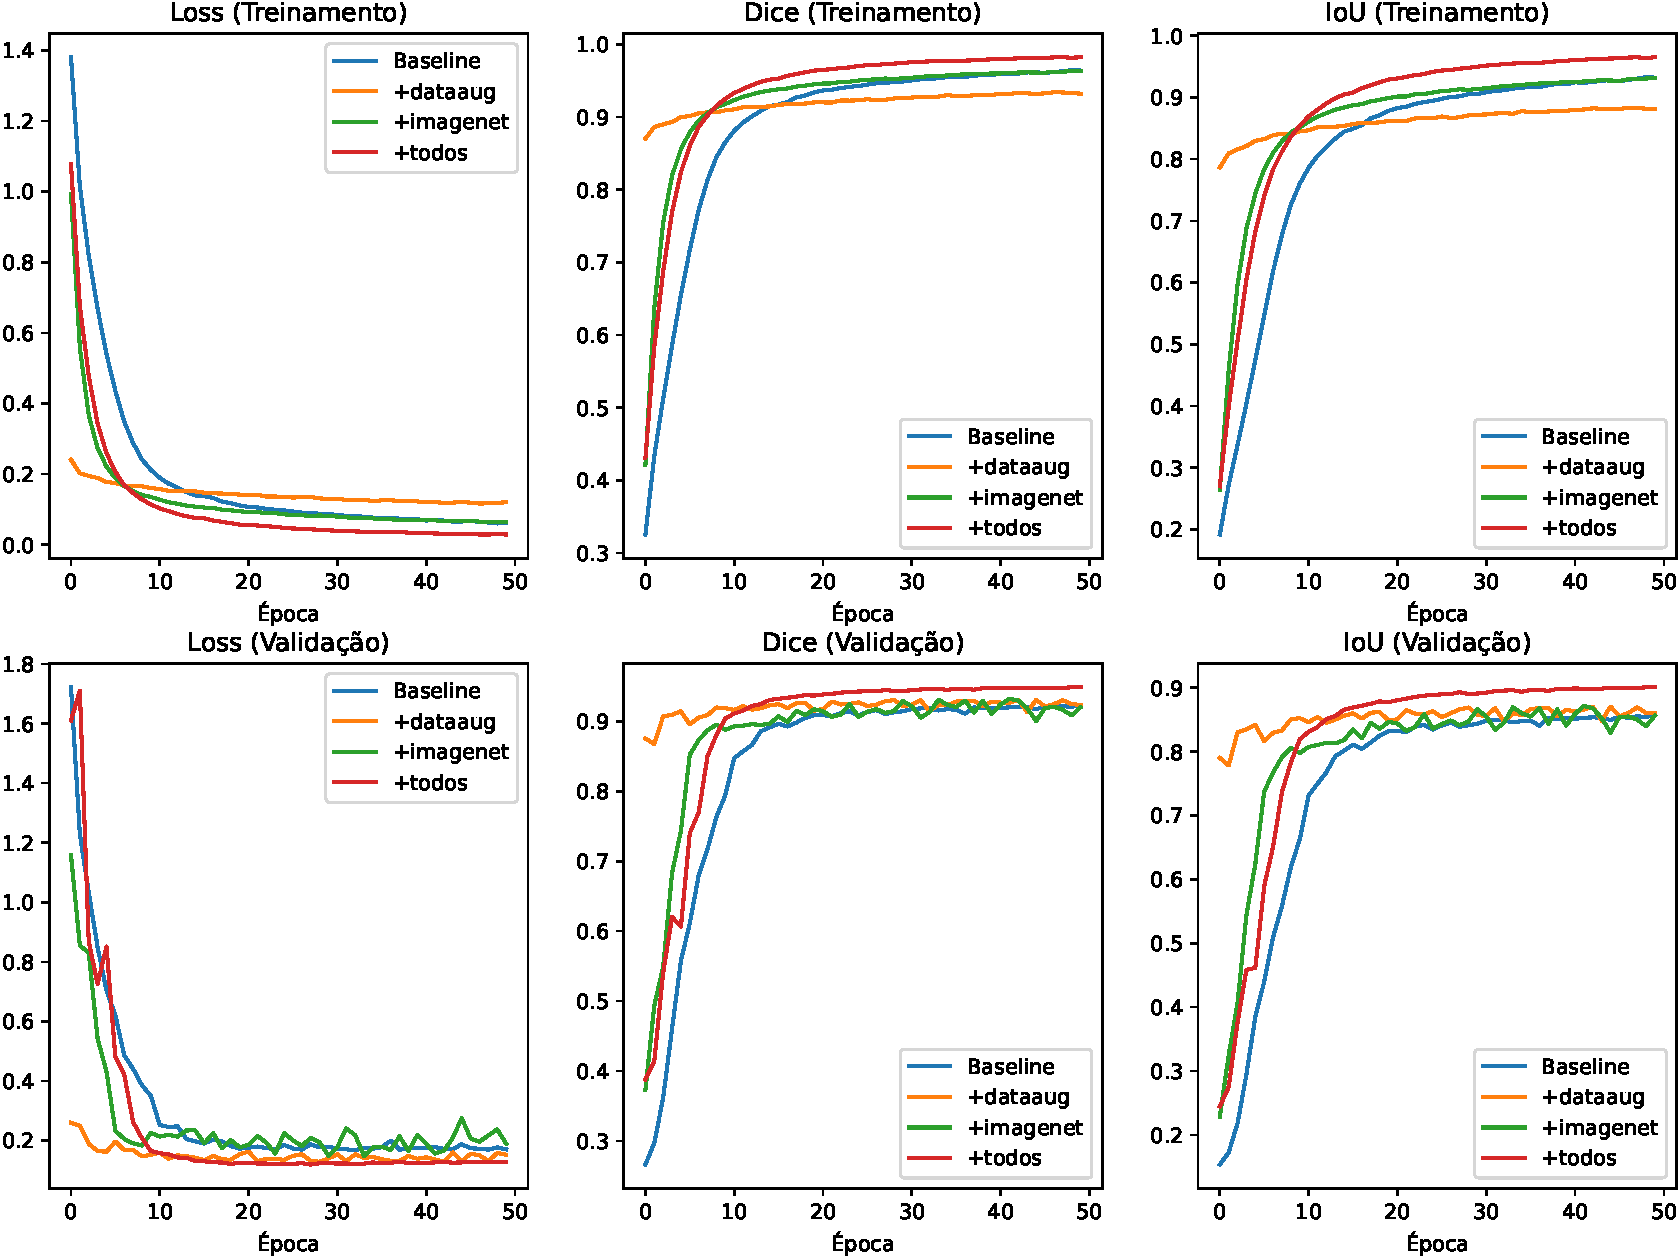
\includegraphics[width=\textwidth]{figures/eval.pdf}
  \caption{Evolução do treinamento comparada com o conjunto de validação}
  \label{fig:eval}
\end{figure}

Para visualização dos resultados, a Fig. \ref{fig:test} mostra segmentações aleatórias feitas pelo modelo, comparadas com os valores de referência.

\begin{figure}[!ht]
  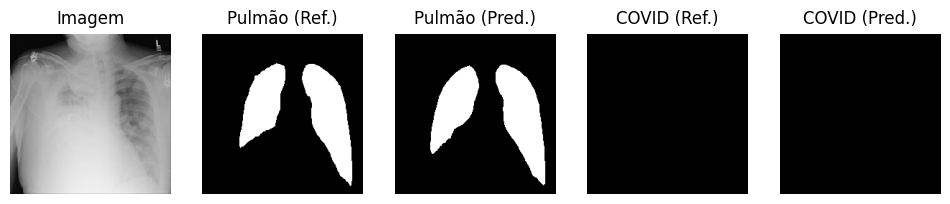
\includegraphics[width=\textwidth]{figures/plot_1.png}
  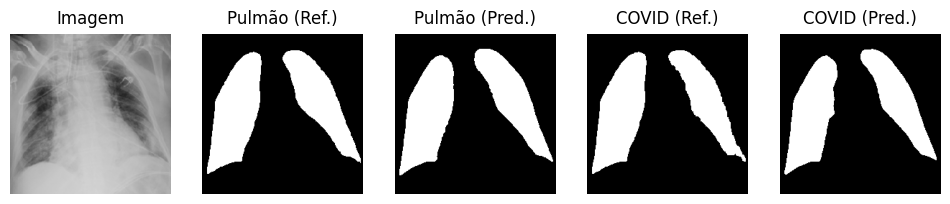
\includegraphics[width=\textwidth]{figures/plot_4.png}
  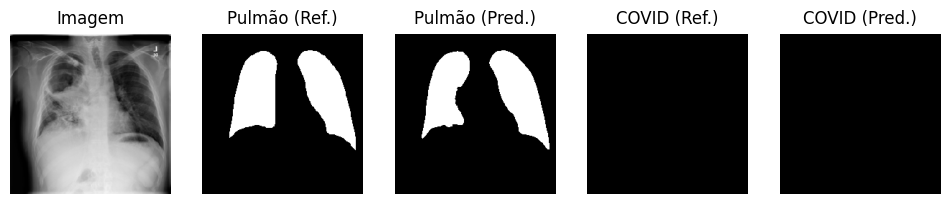
\includegraphics[width=\textwidth]{figures/plot_2.png}
  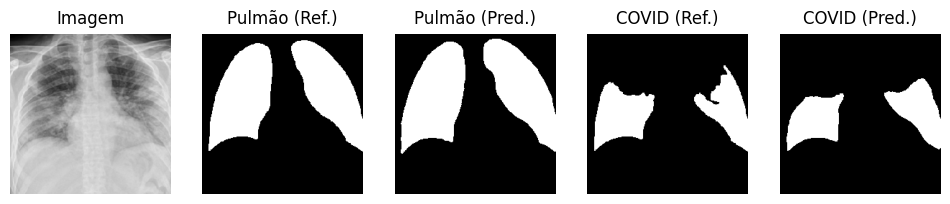
\includegraphics[width=\textwidth]{figures/plot_5.png}
  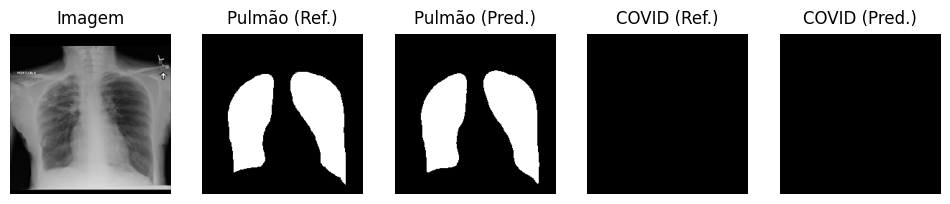
\includegraphics[width=\textwidth]{figures/plot_3.png}
  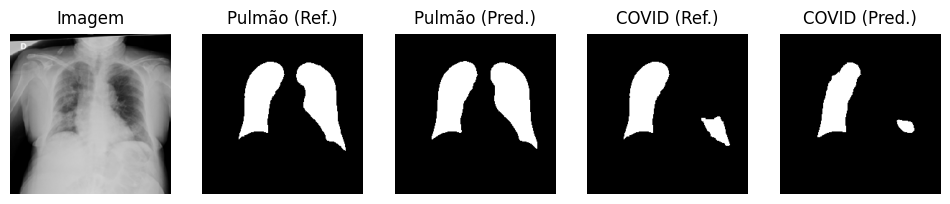
\includegraphics[width=\textwidth]{figures/plot_6.png}
  \caption{Predições no conjunto de teste}
  \label{fig:test}
\end{figure}

\newpage
A Tabela \ref{tab:sumario} sumariza o desempenho do modelo no conjunto de teste. O modelo em que é aplicado tanto transferência de aprendizagem (Seção \ref{sec:tl}) quanto aumento artificial de dados (Seção \ref{sec:dataaug}) apresenta melhor desempenho em todas as métricas.

\begin{table}[!ht]
  \centering
  \caption{Sumário das métricas para os diversos modelos}
  \label{tab:sumario}
  \begin{tabular}{rlllll}
    \toprule
    Modelo    & Loss         & Dice         & IoU          & SSIM (Pulmão) & SSIM (Covid) \\
    \hline
    Baseline  & 0.1820       & 0.9111       & 0.8386       & 0.8870        & 0.8151       \\
    +Data Aug & 0.1280       & 0.9412       & 0.8863       & 0.8960        & 0.8552       \\
    +Imagenet & 0.14922      & 0.9296       & 0.8674       & 0.9123        & 0.8787       \\
    +Todos    & {\bf 0.1278} & {\bf 0.9412} & {\bf 0.8863} & {\bf 0.9135}  & {\bf 0.8846} \\
    \bottomrule
  \end{tabular}
\end{table}








\section{Discussão e Conclusão}
O trabalho realizado demonstrou a eficácia de utilizar redes neurais convolucionais, especificamente a arquitetura UNet, combinadas com a técnica de transferência de aprendizagem para a tarefa de segmentação de imagens de raio-X do pulmão. A utilização de pesos pré-treinados na base ImageNet mostrou-se vantajosa, permitindo uma melhoria significativa nos resultados de segmentação, principalmente em contextos de dados limitados. O uso de técnicas adicionais, como aumento de dados e regularização com dropout, contribuiu ainda mais para a otimização do modelo, refletindo em métricas de desempenho superiores. Estes resultados ressaltam a importância das abordagens utilizadas, especialmente em aplicações críticas como a detecção de condições pulmonares, incluindo a COVID-19. No futuro, investigações adicionais podem explorar a generalização destas técnicas para outras modalidades de imagens médicas e para outras arquiteturas de redes neurais, visando sempre melhorar a acurácia e a robustez dos modelos.


\printbibliography

\horizonBackCover
\end{document}
